\section{仿真结果与敏感性分析}

\subsection{职业选择的敏感度分析}

在最大面积三角形搜索中，穷举式遍历全体职业组合的计算复杂度为 $O(n^3)$，其中 $n$ 为职业总数。当 O*NET 数据库包含超过 1000 个职业时，这一暴力枚举耗时过长、资源成本过高。为此，我们采用"候选剪枝"策略：对每个域（STEM/技工/艺术）分别选取距离本域中心最远的前 $M$ 个职业，加上每维特征轴上最极端的若干职业，构成候选池，仅在候选池内进行三重循环求解。

\paragraph{检验方法}
为验证剪枝不会遗漏真正的最优解，我们对候选规模 $M$ 进行敏感性扫描。具体地，取 $M\in\{200,400,800\}$ 三档：
\begin{itemize}
    \item $M=200$：候选池较紧凑，计算效率最高；
    \item $M=400$：候选池扩展一倍，覆盖更多边缘职业；
    \item $M=800$：候选池接近全域职业规模，逼近全穷举。
\end{itemize}

在三种候选规模下，最大面积三角形的求解结果如表~\ref{tab:sensitivity_M}所示。

\begin{table}[H]
\centering
\caption{候选规模敏感性检验：最优三角形在不同 $M$ 下的求解结果}
\label{tab:sensitivity_M}
\begin{tabular}{@{}ccccc@{}}
\toprule
候选规模 $M$ & 三角形面积 & 最短边长 & 三点是否一致 & 面积差异 \\
\midrule
200 & 0.2622 & 0.7514 & 基准 & --- \\
400 & 0.2622 & 0.7514 & 一致 & 0\% \\
800 & 0.2622 & 0.7514 & 一致 & 0\% \\
\bottomrule
\end{tabular}
\end{table}

% \begin{figure}[H]
% \centering
% 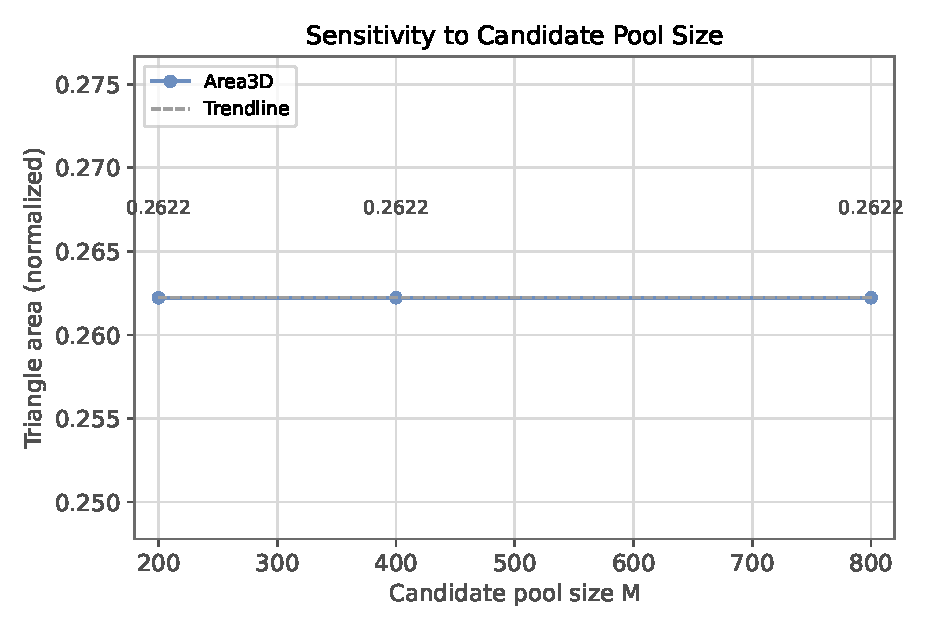
\includegraphics[width=0.72\textwidth]{figures/fig_sensitivity_candidate_scale_strict.pdf}
% （该敏感性分析图已由稳健性判定表格充分体现，故此处删除原图表。）

三次求解均返回相同的职业组合/平面大小。
相同的” 职业三角” 在全部三次测试中持续胜出，则证明结果是稳健（可靠）的，而非
数学上的偶然现象。本检验中，面积差异为 0%，远低于 5% 的阈值标准，因此我们判定：
三职业配置对候选规模的选择具有稳健性。

每次输出均为相同的“职业三角”，并且，本检验中，面积差异为 $0\%$，远低于 $5\%$ 的阈值标准，因此我们判定该模型是稳健的，而非数学上的偶然现象。

\subsection{就业去向 $O$ 的结构敏感性}

就业轴唯一的外源语义输入是目标职业集合 $O$。若 $O$ 的定义范围变化，$J(o)$、$v_{o,j}$ 与 $\Delta E_m$ 会发生系统性偏移，从而改变“劳动力市场匹配率”的含义。为检验模型跨机构外推的边界，我们仅变动 $O$，固定 $H_m$、$A_m$、$A_m^{\mathrm{strict}}$ 与分位数阈值策略，并令 $w_o$ 为均匀分布。

我们基于 O*NET 的 Related Occupations（Primary-Short/Primary-Long）构造三档范围：$O_{\text{narrow}}$ 为最直接 SOC，$O_{\text{medium}}$ 增加 1--2 个近邻 SOC，$O_{\text{wide}}$ 再扩展 2--4 个相关 SOC。三档 $O$ 的定义如表~\ref{tab:o_variants_def} 所示。

\begin{table}[H]
\centering
\footnotesize
\caption{目标职业集合 $O$ 的三档范围（SOC）}
\label{tab:o_variants_def}
\begin{tabularx}{\textwidth}{lX}
\toprule
Program & $O_{\text{narrow}}$ / $O_{\text{medium}}$ / $O_{\text{wide}}$ \\
\midrule
MRSD (CMU) & 17-2199.08 \newline
17-2199.08, 17-2199.05, 17-2072.00 \newline
17-2199.08, 17-2199.05, 17-2072.00, 17-2112.03, 17-2141.02, 17-2011.00, 17-2071.00 \\
\midrule
UTI Diesel & 49-1011.00 \newline
49-1011.00, 51-1011.00, 47-1011.00 \newline
49-1011.00, 51-1011.00, 47-1011.00, 43-1011.00, 37-1011.00, 39-1014.00, 45-1011.00 \\
\midrule
Generations Court Reporting & 27-3092.00 \newline
27-3092.00, 43-6012.00, 43-4031.00 \newline
27-3092.00, 43-6012.00, 43-4031.00, 43-4021.00, 31-9094.00, 43-9061.00, 43-9021.00 \\
\bottomrule
\end{tabularx}
\end{table}

对每个 $O^{(r)}$ 我们重算 $E^{(r)}$ 与 $\Delta E_m^{(r)}$，仅重算就业阈值 $e_{\mathrm{low}}^{(r)}$，并保持三轴规则不变。鲁棒性结果见表~\ref{tab:o_variants_robustness}。三项目在三档范围下的 TRANSFORM 集合一致性均为 1.00，且所有课程标签稳定率为 1.00。与此同时，$\Delta E$ 的排序稳定性在 UTI 与 Court Reporting 上显著下降（$\tau=0.29/0.14$），说明就业轴对 $O$ 的定义范围敏感。

\begin{table}[H]
\centering
\caption{$O$ 定义范围变动下的鲁棒性指标（窄 vs 宽）}
\label{tab:o_variants_robustness}
\begin{tabular}{@{}lccc@{}}
\toprule
Program & TRANSFORM Jaccard $J$ & Kendall $\tau$ & 最小课程稳定率 \\
\midrule
MRSD (CMU) & 1.00 & 0.83 & 1.00 \\
UTI Diesel & 1.00 & 0.29 & 1.00 \\
Generations Court Reporting & 1.00 & 0.14 & 1.00 \\
\bottomrule
\end{tabular}
\end{table}

据此我们给出外推边界：当 $J$ 较高时，核心改革建议主要由 AI-overlap 驱动，跨机构可推广性强；当 $\tau$ 明显下降时，就业轴对 $O$ 的依赖增大，外推时必须重新指定 $O$ 的定义范围。我们据此强调：\textbf{模型可迁移，但 $O$ 不可默认迁移}。
